\section{Funciones}

Una \textbf{función} es un bloque de código que realiza una tarea particular, esta tarea es ejecutada cuando se le "llama" a la función para que ejecute sus instrucciones. Su estructura es la siguiente:
\begin{lstlisting}
    function nombre (parámetros) {
        // Código.
    }
\end{lstlisting}

Los nombres de funciones siguen las mismas reglas que los nombres de variables. Las funciones se pueden llamar simplemente escribiendo su nombre, seguido por paréntesis o por un punto y la función \textbf{call()}:
\begin{lstlisting}
    function hola () {
        console.log("hola mundo")
    }

    hola()
    hola.call()
\end{lstlisting}


\subsection{Parámetros}

Son valores que recibe la función y que pueden ser utilizados por la misma para realizar su tarea. Su estructura es la siguiente:
\begin{lstlisting}
    func// Código.
    }
\end{lstlisting}

En caso de que se llame a una función y no se le pasen la cantidad de parámetros que posee (se le pasan dos en vez de tres), aquellos que no recibieron un valor pasan a ser \textbf{undefined}. Vemos entonces que los parámetros, al igual que las variables, \textbf{no requieren de indicar su tipo de dato}.


\subsection{Sentencia return}

La palabra reservada \textbf{return} es utilizada para regresar un valor de una función, una vez que el lenguaje encuentra esta palabra en una función, acaba la ejecución de la misma. Veamos un ejemplo:
\begin{lstlisting}
    function alCubo (num) {
        return num * num * num;
    }

    console.log(alCubo(3))
\end{lstlisting}

En caso de que haya un error regresando un valor o variable, o esta variable no tenga ningún valor, lo que regresará la función es \textbf{undefined}.


\subsection{Funciones Alert, Prompt y Confirm}

La función \textbf{alert()} muestra una caja con un mensaje en el sitio web, el único parámetro que recibe es una cadena, la cual muestra al usuario, y posee un único botón para interactuar, el cual dice OK, como se ve en la \textit{Figura \ref{fig: 1}}.
\begin{figure}[H]
    \caption{Ejemplo de la función alert()}
    \label{fig: 1}
    \begin{center}
        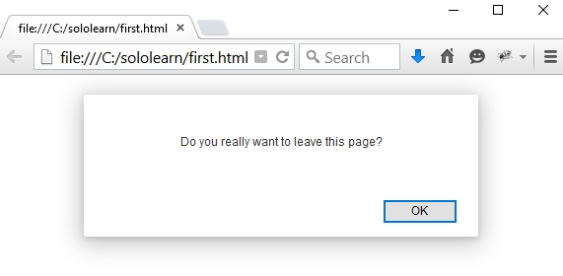
\includegraphics [width=9cm]{ss/alert.png}
    \end{center}
\end{figure}

La función \textbf{prompt()} muestra una caja con un mensaje en el sitio web, y solicita al usuario que ingrese alguna información; posee dos parámetros: el primero es el mensaje a mostrar en la caja y el segundo es un texto por defecto dentro de la caja de texto que posee la caja; posee dos botones: el botón OK, si es presionado, la función regresa lo que el usuario ingresó, y el botón Cancel, que cierra la caja y regresa null, como vemos en la \textit{Figura \ref{fig: 2}}. No se recomienda utilizar demasiado esta función.
\begin{figure}[H]
    \caption{Ejemplo de la función prompt()}
    \label{fig: 2}
    \begin{center}
        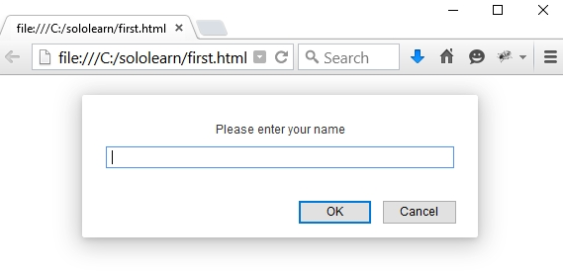
\includegraphics [width=9cm]{ss/prompt.png}
    \end{center}
\end{figure}

La función \textbf{confirm()} muestra una caja con un mensaje en el sitio web, muestra un mensaje que el usuario debe confirmar para continuar; esta caja posee dos botones: el botón OK, si es presionado, la función regresa true, y el botón Cancel, que cierra la caja y regresa false; la \textit{Figura \ref{fig: 3}} muestra como se ve inicialmente la caja de confirm().
\begin{figure}[H]
    \caption{Ejemplo de la función confirm()}
    \label{fig: 3}
    \begin{center}
        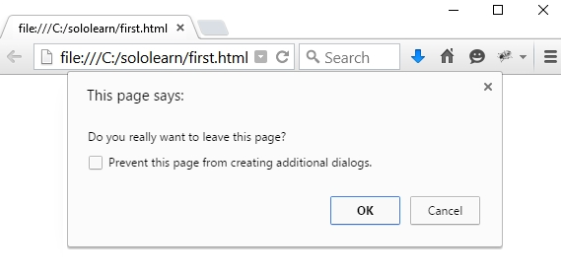
\includegraphics [width=9cm]{ss/confirm.png}
    \end{center}
\end{figure}

No es recomendado utilizar demasiado este método, porque impide que el usuario interactúe con el sitio hasta que de clic en alguno de los botones de la caja; la \textit{Figura \ref{fig: 4}} muestra la caja cuando se le da clic al botón OK.
\begin{figure}[H]
    \caption{Mensaje cuando se presiona botón OK de la función confirm()}
    \label{fig: 4}
    \begin{center}
        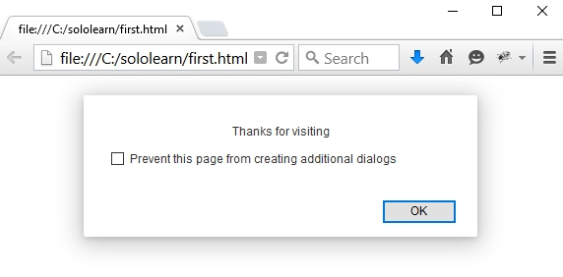
\includegraphics [width=9cm]{ss/confirm_res.png}
    \end{center}
\end{figure}


\subsection{Función setInterval}

Esta función llama a una función o evalúa una expresión cada determinado tiempo (en milisegundos), seguirá llamando o evaluando hasta que se ejecute la función \textbf{clearInterval()}, como vemos enseguida:
\begin{lstlisting}
    // Declara función para mostrar en ventana un mensaje.
    function miAlerta() {
        alert("Hola mundo");
    }

    // Llama a la función setInterval que llama a la función miAlerta
    // cada tres segundos.
    setInterval(miAlerta, 3000);
\end{lstlisting}

Nótese que, dentro de los parámetros de \textit{setInterval()}, la función a llamar no posee paréntesis al final de su nombre. Para el caso anterior, la función setInterval no detendrá su ejecución porque no está la instrucción \textit{clearInterval()} ni aunque se presione el botón OK de la caja.
